% !TeX root = ../main.tex
% Add the above to each chapter to make compiling the PDF easier in some editors.

\section{Monoscopic Far-Field Rendering} \label{MFFR}
Monoscopic Far-Field Rendering (\gls{MFFR}) is an approach strongly leaning toward an inherent property of many optimizations in the field of rendering and real-time computing in general, which is the property of trading accuracy for speed. \gls{MFFR} is a topic brought up again soon after Oculus Rift CV1's retail launch by Oculus developers Rémi Palandri and Simon Green at developer keynotes like the ARM GDC 2017 talk\cite{DiDonato.01.03.2017} and the Oculus Developer Blog as Hybrid Mono Rendering\cite{Palandri.2016}. \\
Understanding the concept requires some explanation of the technical and visual background. Depth perception of the human eye relies on the slight spatial distance between both eyes as each eye sees a slightly different angle of a given object. This difference in perceived angle is called stereo separation. Without it, the brain has difficulties determining the depth at which a certain object or surface lies. Regular stereo rendering recreates this separation correctly when rendering the two virtual eyes at their respective spatial offset from the \gls{HMD} center - given correct projection and view matrices and accurate world scale at least. \\

However, as distance grows, stereo separation shrinks - the aspect \gls{MFFR} exploits. In infinity, separation would be infinitely small. Even at more reasonable distances separation is small enough so even with good vision it is hard to properly judge depth unless the object is large. This of course also holds true for rendered stereoscopy, but an additional limit is the pixel density of the output displays. This means that at a certain distance from the virtual camera, stereo separation will shrink to less than a full screen space pixel once projected. If the difference can not physically be displayed by the \gls{HMD}, it is a waste of resources to still render both eyes. \\
Mono Far-Field Rendering opts to skip the second view during rendering of the name-giving far field of objects. The hope here is to only render a single view past a certain distance, reducing rendering load without the user noticing the theoretical loss in accuracy. 
This approach has caveats however. The value at which a field split - the distance at which the stereo rendering is cut off and followed by only mono rendering - will depend on the individual user, their quality of vision and spatial awareness. It will also potentially depend on the resolution of the used headset given the user's vision is good enough to not deteriorate before that point. Note here, this thesis will not explore these constraints of \gls{MFFR} further than approximate values used for testing as time does not allow more. \\
\gls{MFFR} has been implemented by Oculus LLC and Epic Games Inc in Unreal Engine 4 and was recommended for certain types of pixel-bound mobile \gls{VR} experiences with very limited GPU power but  has been removed from the engine in update 4.20 without further explanation. An odd decision, as UE documentation posts prior to the removal indicated continued optimization efforts such as added compatibility with UE4's multiview path\cite{EpicGamesInc..2016}. 

\begin{figure}[htb]
  \centering
  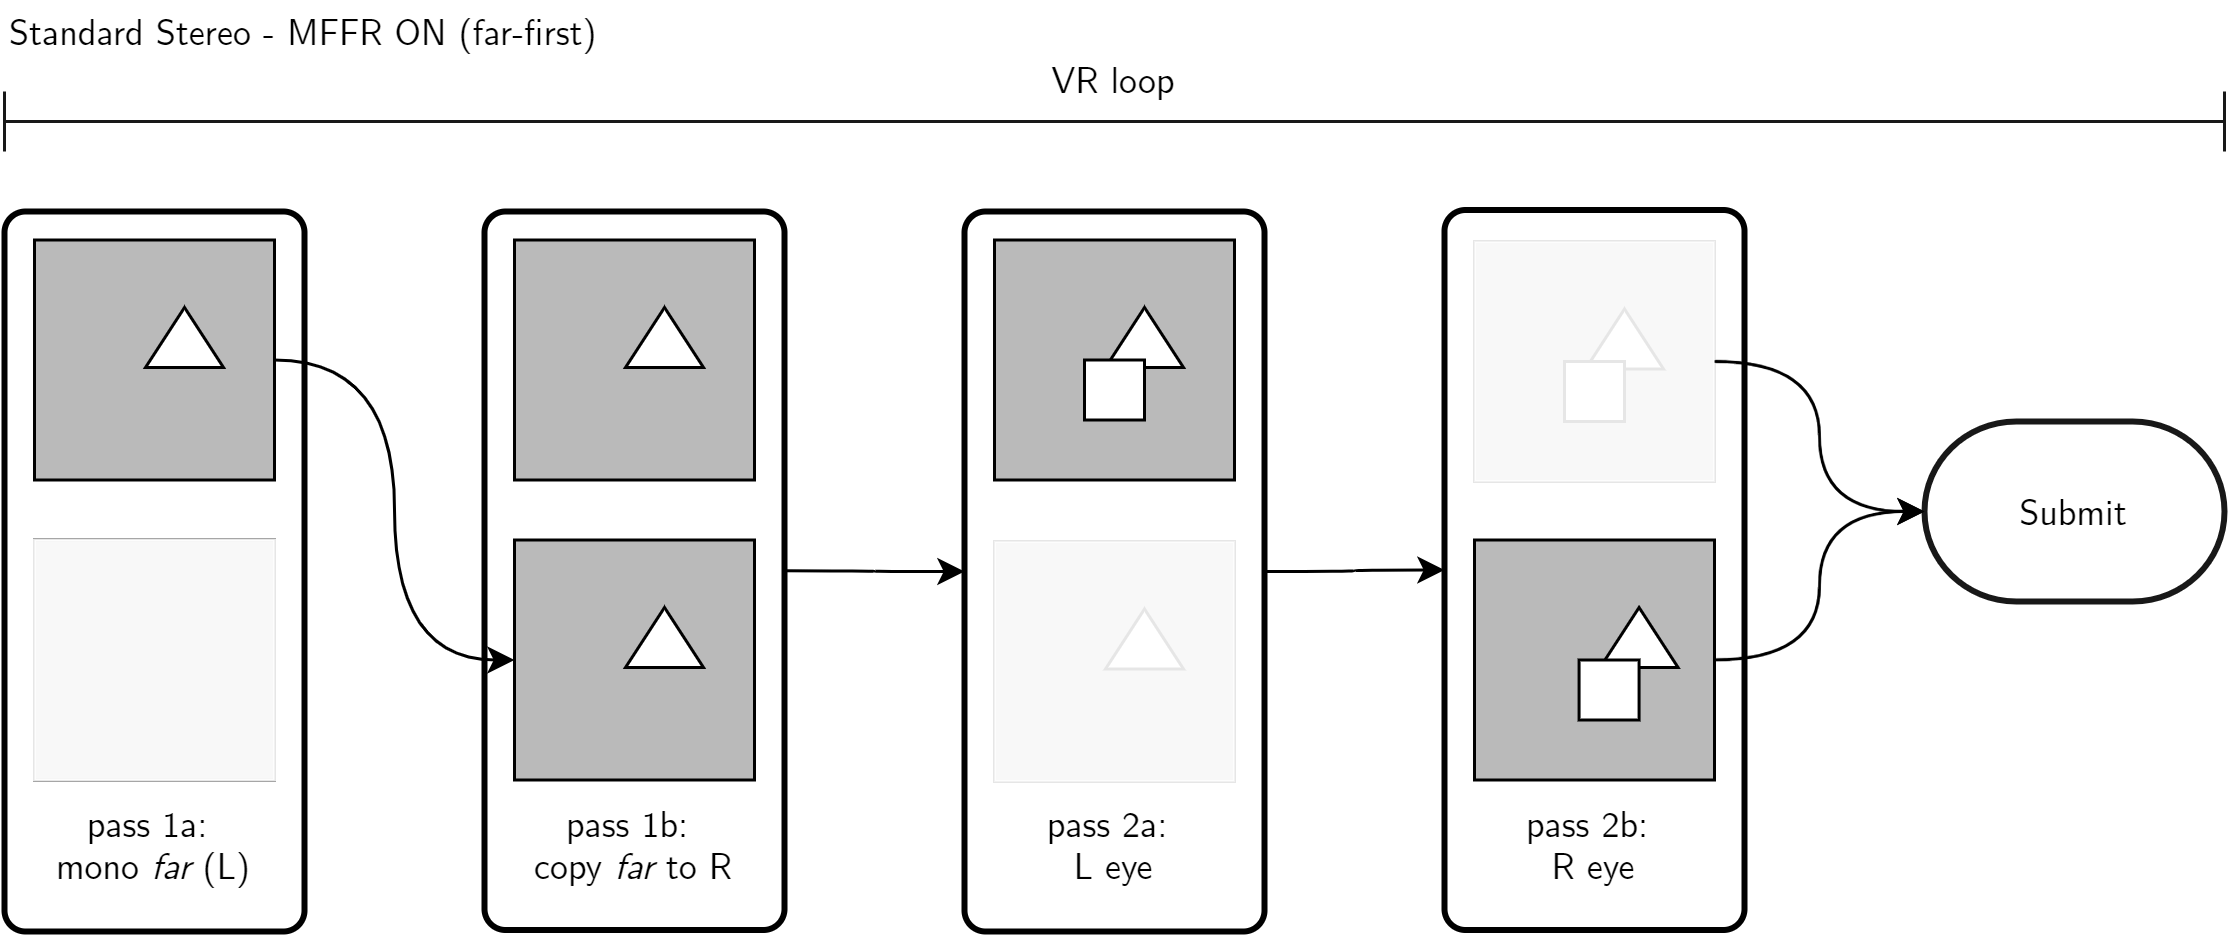
\includegraphics[width=0.9\textwidth]{pictures/MFFR_farfirst}
  \caption{Per-frame render pass flow of far-first \gls{MFFR}; \\
  Each row represents one image buffer, each column represents the process steps the respective buffer is subjected to} \label{fig:flowchart_MFFR_FarFirst}
\end{figure}

\subsection{Estimated impact}
The makeup of the scene itself will also affect the effectiveness of the solution. As cautioned by Oculus LLC in their developer reference on Mono Far-Field Rendering \cite{Palandri.2016}, there is a certain baseline overhead simply for enabling the additional render pass necessary for the monoscopic image and the associated context switches. Furthermore, only scenes with a significant amount of distant geometry beyond the field split distance will benefit from the optimization, as obviously the second view workload can only be saved for objects originally contained within that second pass. \\
Going purely by Palandri and Green's blog entry, their forward-rendered UE4 implementation supposedly running on a GearVR device saw frametimes in the Epic SunTemple sample scene drop by 25\% and their best-case Unity test scene demonstrated a 49\% drop\cite{Palandri.2016}. 
This would indicate that if circumstances allow - meaning pixel-bound forward-rendered large scale scenes - impressive performance gains well upwards of 20\% can be expected, while less suitable cases in the worst case will see no change if not minor regression. 

\subsection{Far-first approach}
Implementing Mono Far-Field Rendering into \gls{Tachyon} - or any renderer for that matter - requires care and a number of changes. There are at least two possible ways of doing it, both by way of multiple render passes and with their own respective drawbacks and advantages. One way of implementing \gls{MFFR} is doing the far pass first in each frame, followed by a near pass, both possibly using the same framebuffer as illustrated in \autoref{fig:flowchart_MFFR_FarFirst}. At the start of the frame, the framebuffer is cleared - color and depth clear are necessary - after which the far-field command buffers are submitted and executed. This pass can render directly into the buffer of one eye and copy color and depth buffer to the other eye. Finally, the near-field command buffers are submitted and render their values into the buffers already containing the far field information. For this case, one extra step needs to be performed. As the projection matrix normally projects the world as seen by the camera into a uni-cube with each axis being length 1 going from 0 to 1 and this same uni-cube is used for both depth value calculation and projection clipping (triangle discard via clip space evaluation), the two passes can not share the same uni-cube. Ways around this would be to either use regular full-depth projection matrices and clear the depth buffer before the near pass or to scale both passes' projection matrices by 0.5 and translate the far projection by 0.5 so the uni-cube is shared between the two fields without overlap. \\
If neither is done, the effective depth values of far-pass objects will be closer than they should be and possibly closer than those of near-pass objects, leading to some near-field objects being drawn behind far ones. 
The depth buffer clear option has the benefit of utilizing full projection precision and correct triangle clipping. The matrix squashing option avoids an extra clear but means vertices otherwise clipped outside of the uni-cube are pulled into the uni-cube and not skipped. \\
The overall advantage of this far-first approach is it yields a full precision far-field depth buffer which may be useful for stereo interpolation as briefly described in the \autoref{MFFR_depthshift}. The disadvantage is early Z discard cannot be fully effective as all far geometry is rendered first even if opaque geometry close to the camera would later obstruct it. Whether the benefits of lower split distance coupled with interpolation can outweigh the additional cost of overdraw heavily depends on the scene and how much geometry is contained within the far volume. 
The goal of this approach is to reduce memory operations and locality to a minimum and avoid more costly compositing methods. 

\subsection{Near-first approach}
The alternative to rendering the far pass first is to render the stereo near volume at the start of each frame as illustrated in \autoref{fig:flowchart_MFFR_NearFirst}. A key difference to the former approach is the first pass needing to flag the stencil buffer pixel when an opaque fragment is within the uni-cube and a color value is written. After the stereo pass, each eye contains a binary stencil mask of the near-field occluded screen areas. In the next step, the far pass can then execute regularly except with stencil testing enabled. This sequence has no direct need for depth buffer clearing or uni-cube sharing. However, the constraint is the far pass also needing to sample from left to right eye separately as a straight buffer copy cannot work anymore. 
The advantage of this approach over far-first is early Z discard takes full effect and stencil masking reducing the leftover render area even more. The downside is the need to perform additional stencil writes every frame and potentially costly sampling operations.

\begin{figure}[htb]
  \centering
  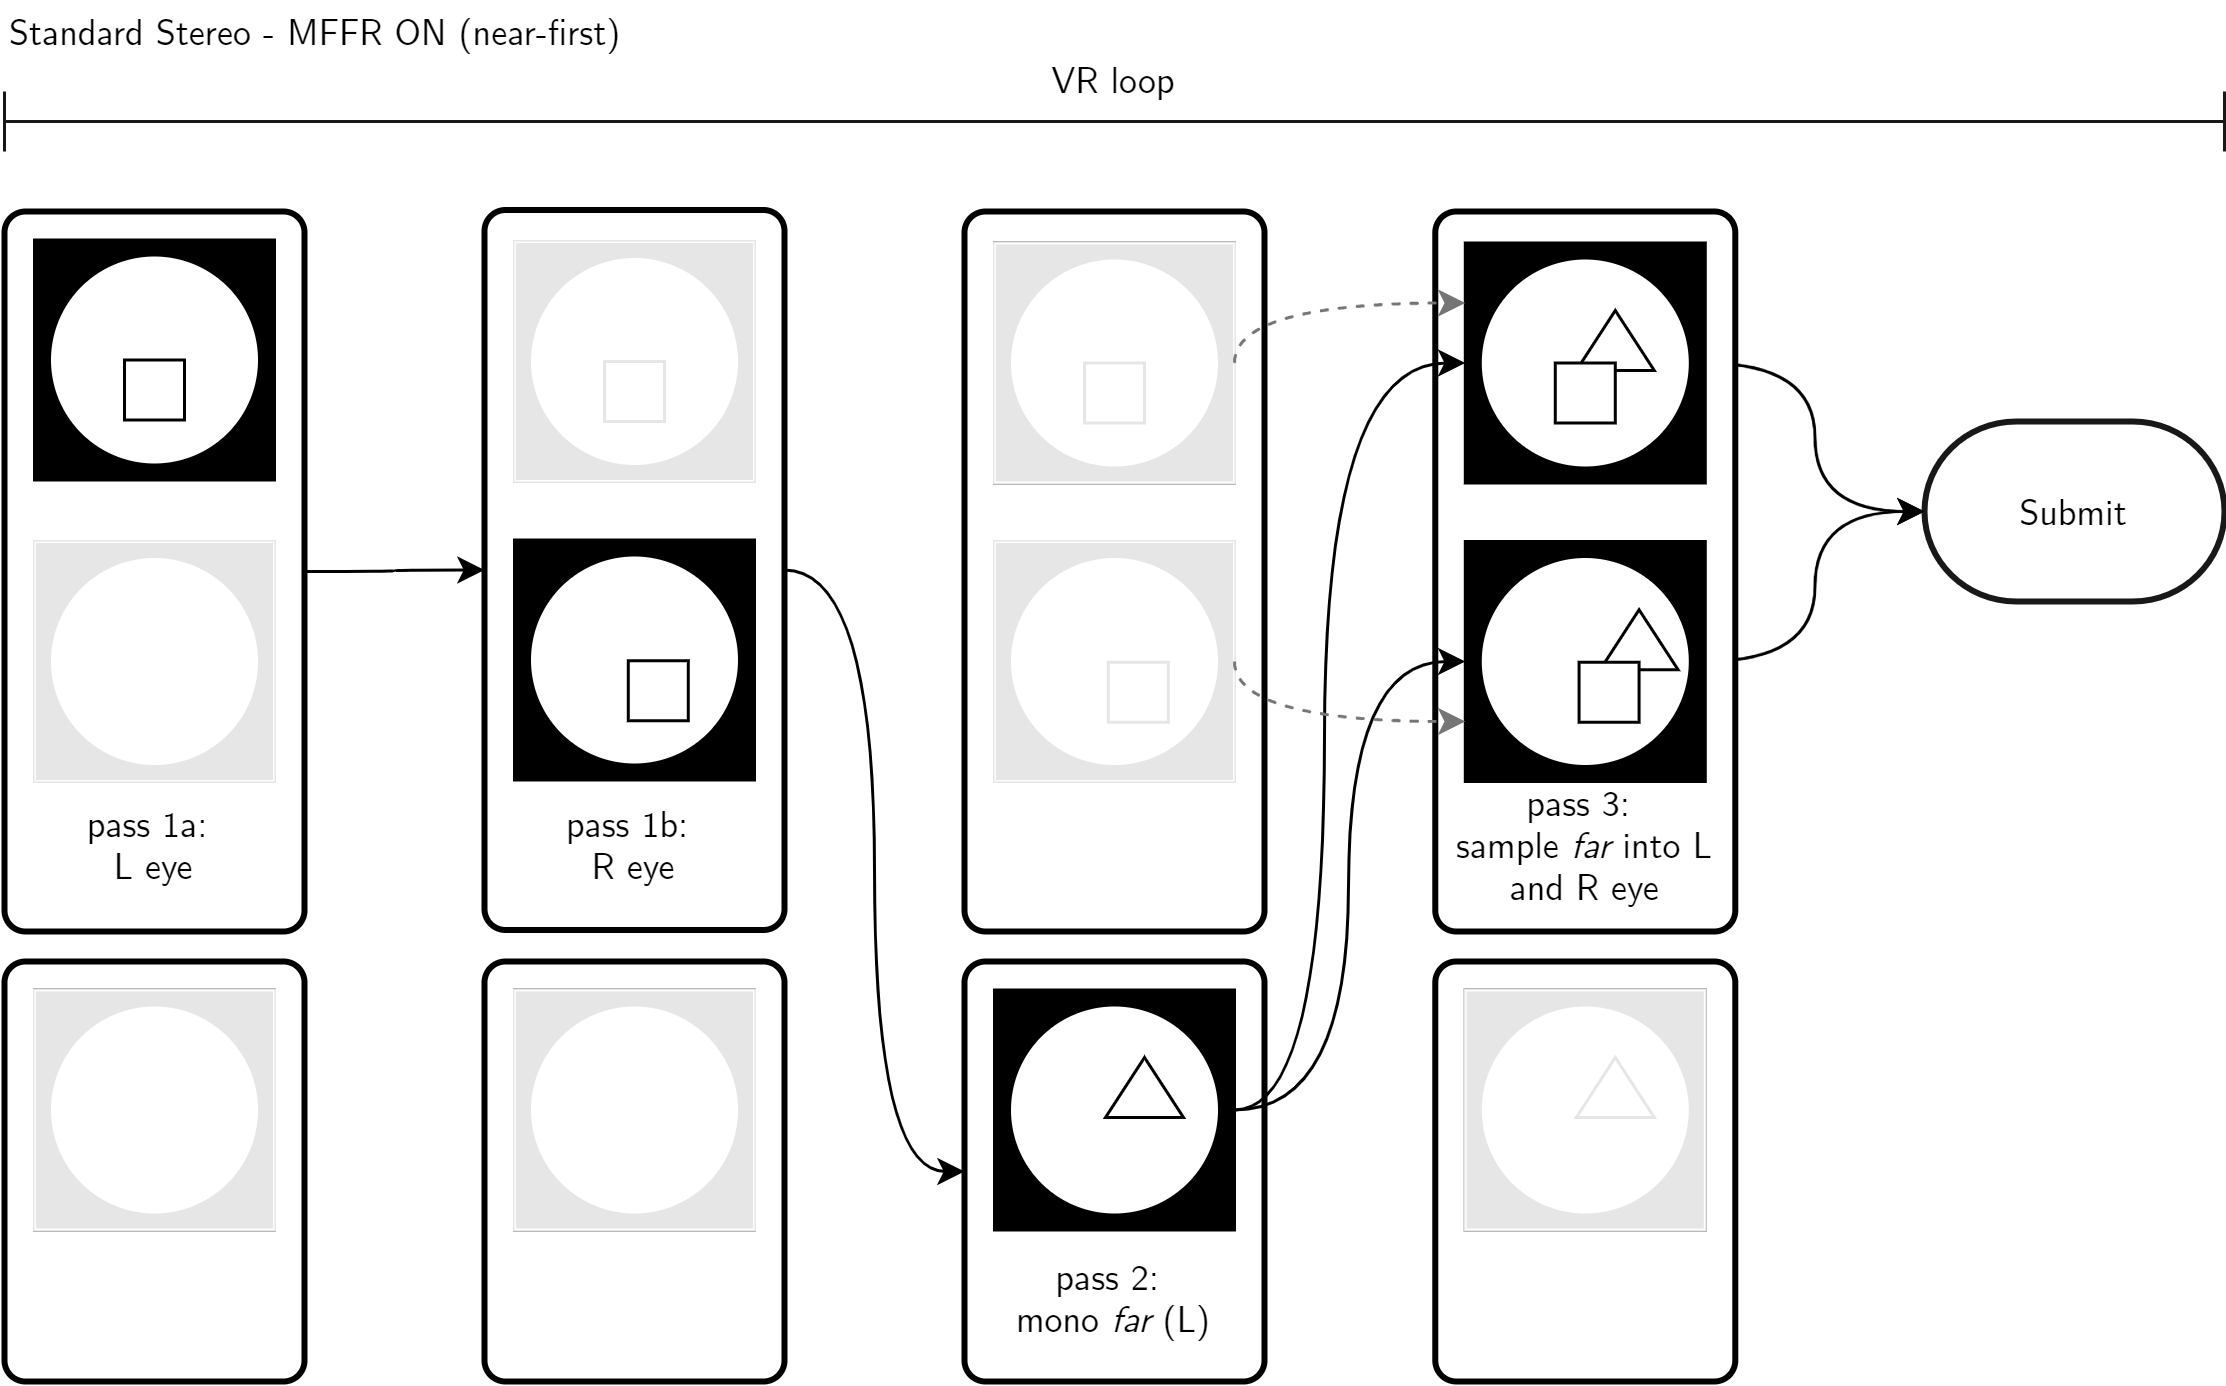
\includegraphics[width=0.9\textwidth]{pictures/MFFR_nearfirst}
  \caption{Per-frame render pass flow of near-first \gls{MFFR}; \\
  Each row represents one image buffer, each column represents the process steps the respective buffer is subjected to} \label{fig:flowchart_MFFR_NearFirst}
\end{figure}
 
\subsection{Implementation specifics}
In this thesis, the plan is to do far-first \gls{MFFR}, albeit the measured results are not favorable. In the first step of each \gls{VR} frame, a monoscopic render pass renders the far clip volume's color and depth values into the index 0 layer of the framebuffer. The next step is to copy that layer to index 1 as well. In the final step the regular stereoscopic render commands are executed with reduced near field clip volume, including clearing the depth buffer at the start of the stereo pass to avoid the uni-cube issue. 
While the general approach is mostly straight-forward and both described ways are possible, implementing either in a Vulkan renderer is no trivial task and requires the following changes to \gls{rtvklib}: 
\begin{itemize}
\item for the virtual camera, a field split distance parameter is introduced and an additional frustum is added; the stereo frusta cover the volume from near plane to split plane while the far field frustum covers split plane to far plane
\item the frustum culling procedure is altered to write the far frustum's resulting draw commands into a separate set instead of merging them into one (as would happen for regular multifrustum culling in \gls{Tachyon})
\item at initialization time of the \gls{VR} render target an additional render pass is created for monoscopy with the main difference - compared to the regular \gls{VR} render pass - being the removal of the multiview extension
\item an additional set of Vulkan \codeword{VkCommandBuffer}s is added, into which the draw commands of the far frustum cull set are to be recorded
\item an additional set of \codeword{VkSemaphore}s is added to synchronize the two render passes and create them in \codeword{CreateSyncObjects()} during initialization
\item an additional \codeword{VkCommandBuffer} for the layer copy operation is added
\item at initialization time of the \gls{VR} render target this copy command buffer is pre-recorded so it can be reused every frame; this recording includes transitioning the layout of both the color and depth image from \codeword{VK_IMAGE_LAYOUT_TRANSFER_SRC_OPTIMAL} to \codeword{VK_IMAGE_LAYOUT_GENERAL}, \codeword{vkCmdCopyImage(...)} both images' layer 0 to layer 1 and then transitioning the layouts in reverse again
\item in the per-frame recording procedure of the \gls{VR} render target, \\\codeword{RecordCommandBuffers(...)}, the entire structure of begin and end of command buffers and render pass and per-pipeline \codeword{RecordDrawCommand(...)} calls is duplicated with the monoscopy render pass and far field command buffers set; afterward the prior regular stereo recording still takes place
\item in the render target's \codeword{RenderFrame(...)} function the far field command buffer and layer copy command buffer submission is inserted before the regular stereo submits; the mono submit is set to wait on \codeword{mRenderCompleteSemaphores} and signal \codeword{mFarfieldCompleteSemaphores}, while the stereo submit is only set to wait on the latter
\item in \gls{VR} render target's camera setup, the far field frustum projection matrix is constructed as outlined in \cite{Lapinski.2017} pp. 515-519 - albeit transposed as \gls{Tachyon} still retains the OpenGL matrix format for a few matrix types
\item an additional set of camera data struct and camera index is added
\item in the render target's \codeword{UpdateCameras()} call, the far field volume's view projection matrix is updated by transforming aforementioned projection matrix by the current \gls{HMD} pose and the updated matrix is written to the camera data buffer on the GPU
\end{itemize}

\subsection{\gls{rtvklib} \gls{MFFR} failure} \label{MFFR_failure}
Some issues with this implementation prevail and make it unfit for productive deployment in \gls{Tachyon}. For one, while the projection matrix itself uses the correct parameters, view matrix transformation used for the far field remains incorrect, so head movement leads to incorrect projection distortion effects on the horizontal axis. While the lack of pure separation at little to no sideways tilt may be acceptable and not easily noticed with a correct view matrix, tilting the head means more severe separation mismatch as the spatial disconnect is expanded from being mostly horizontal to being horizontal and vertical, clearly visible in \autoref{fig:distortion_MFFR}. Fixing this disparity would require translating the far field image of each eye to conform more closely to the expected overall stereo shift. 
Vitally, this visual distortion does not affect performance measurements presented in \autoref{results} as the used internal culling frustum is computed from the virtual camera's world position and direction in any given frame and not subject to incorrect projection transformation. Subsequently, submitted draws and render passes are correct and executed in the described order, as exemplified by the Nvidia \gls{Nsight VS} debug timeline in \autoref{fig:Nsight_MFFR}. 

\begin{figure}[htb]
  \centering
  \includegraphics[width=0.9\textwidth]{pictures/MFFR_timeline_stacked_delimited}
  \caption{Draw submission and render pass binding timeline of a typical \gls{rtvklib} \gls{MFFR} frame, captured in \gls{Nsight VS}. (Split after far-field render pass and stacked vertically for better page fit) \\On the "Render Pass" row, the blue pass denotes the far-field pass, orange is the left eye and green is the right eye. Far and near are each synchronized by a VkSemaphore.} \label{fig:Nsight_MFFR}
\end{figure}

Secondly, Vulkan render passes discard fragments at their end by default if depth testing is enabled and the depth value of said fragment equals 1.0 (and is thus on the far plane). This means any color values written by the far pass and not overwritten by the near pass are discarded right at the end of the stereo pass and before presentation. A workaround for this is to clear the depth buffer at the start of the stereo pass not to 1.0 but to 0.999999, which is the closest value an IEEE-754 float can reach below 1.0 (22 of 23 mantissa bits set to 1). With this tweak, color values were composited together without any visible loss at the near field's split plane, even if it technically entails a depth clamp in that last mantissa bit. \\
Lastly, and most importantly, performance simply is not up to par. On the i7 and RTX2080 test system (\textbf{WS-Big}, see \autoref{benchmark_setup}), enabling \gls{MFFR} with a sufficiently far split distance yielded a 34\% performance loss. The culprit for this is most likely two-fold. One factor is the detrimental Z ordering of the submitted draw commands since much of the far field color buffer is overdrawn by the near pass and thus counts as wasted effort. The other factor is the lack of parallelism due to the use of a shared framebuffer. The two render passes need to be synchronized to run in order and cannot be scheduled on parallel thread warps to increase GPU utilization and thus performance. What's puzzling in this scenario is that Palandri et al. in their Oculus blog entry\cite{Palandri.2016} saw a clear performance uplift in a Unity sample scene with seemingly very similar \gls{MFFR} construction. \\
As such, the \gls{rtvklib} \gls{MFFR} implementation as presented here remains beneficial only in theory and will require further work to result in real performance gain. 

\begin{figure}[h!]
  \centering
  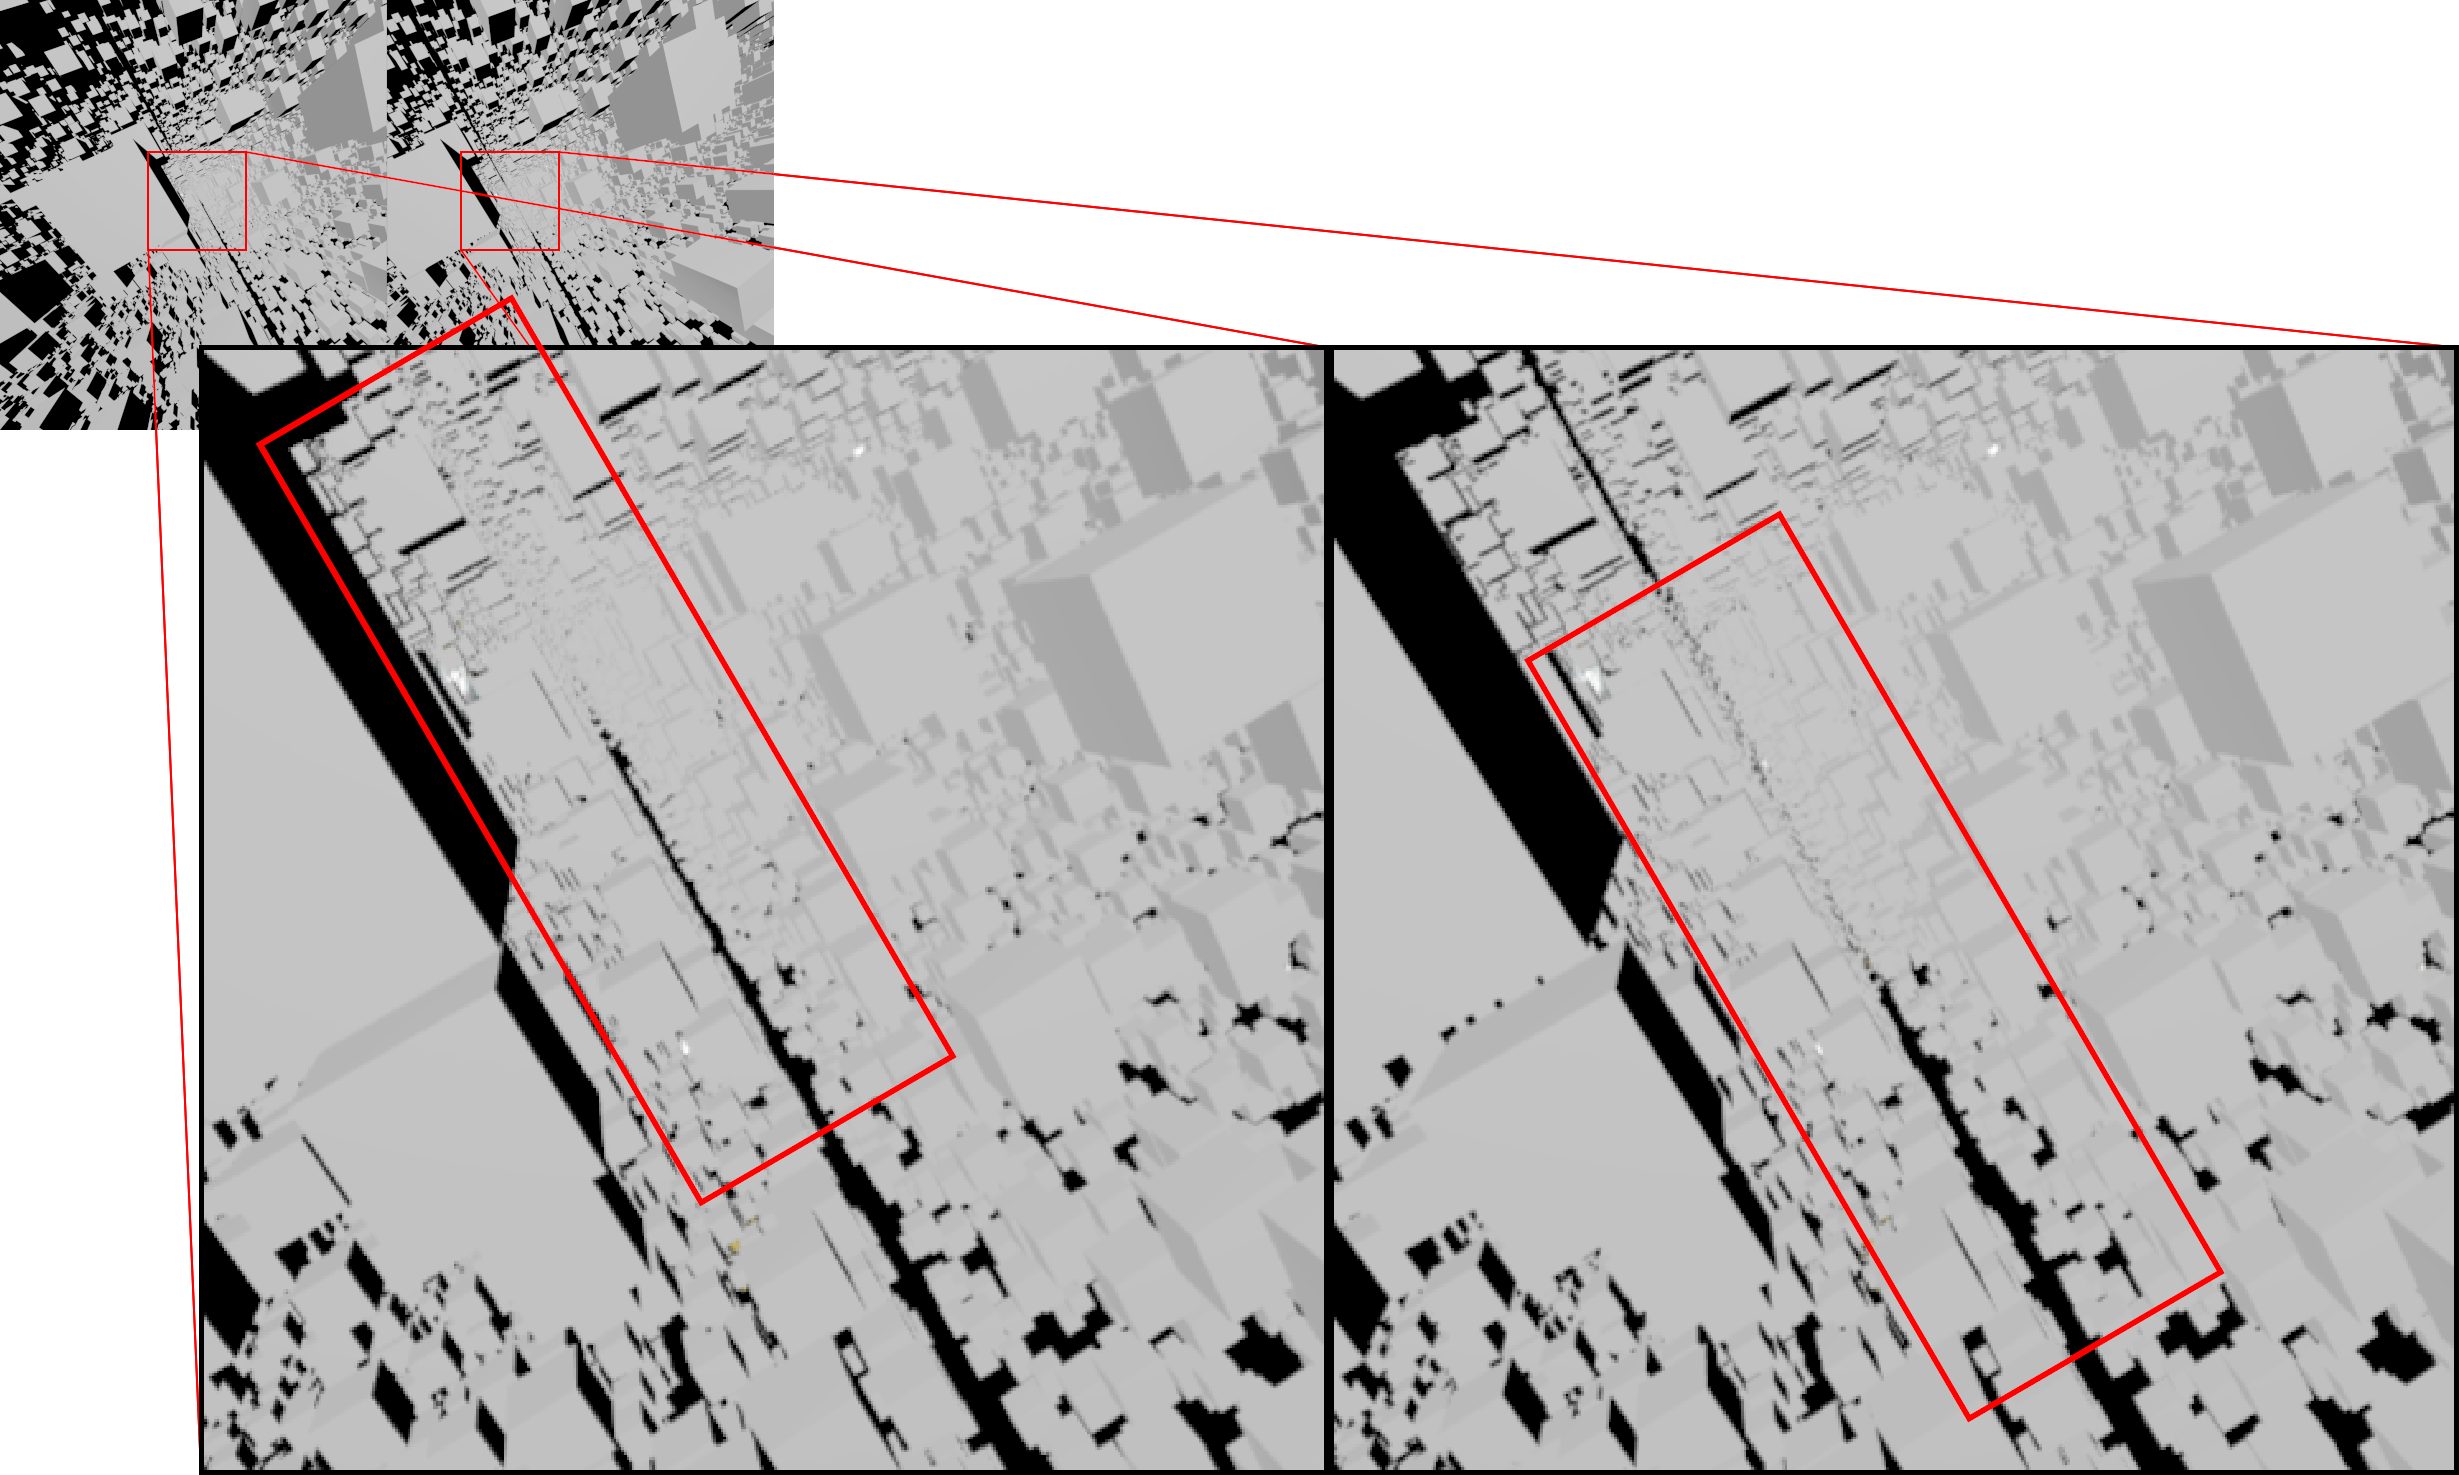
\includegraphics[width=0.9\textwidth]{pictures/mffr_tilt_distortion}
  \caption{Incorrect monoscopic far field distortion (notice the thin center line of distant geometry shifted up and left in the Left Eye image, but shifted down and right in the Right Eye image)} \label{fig:distortion_MFFR}
\end{figure}

\subsection{\gls{MFFR} Variant: Depth Shift}  \label{MFFR_depthshift}
In its basic version \gls{MFFR} as described in \autoref{MFFR} completely foregoes separation beyond the split distance and as such the split distance has to be set relatively far back to minimize the visual inaccuracy. Naturally, an attempt to try and reduce that split distance closer to the camera is by artificially and cheaply increasing that accuracy again. One such way is to use the data already contained in the framebuffer's depth layer during rendering. As stereo separation is mostly dependent on depth, given the object itself and its properties are known, an improvement is to approximate small amounts of separation based on that depth buffer. Instead of simply copying or sampling the far image to both eyes after the far field pass, one can do an additional sampling or post-processing pass which includes slightly shifting pixels according to the depth value of the respective given fragment. \\
This interpolation should allow pulling the field split distance closer to the camera and save some stereo render time, but it is unclear whether the savings outweigh the additional processing cost and this thesis does not explore \gls{MFFR} beyond the base variant. 

\iffalse
\textcolor{red}{[TODO: shift math or geometric illustration]}
\fi

\subsection{\gls{MFFR} Variant: Alternate eye}
Another possible way of pulling in the split distance value while retaining approximated separation comes back to the \gls{VR} property of high framerate as explained in earlier chapters like the Round Robin Culling (\autoref{RRCull}). Assuming high framerate and refresh rate, the mono render pass could be called with the camera parameters not custom calculated as a middle point between the two eyes but alternating between left and right eye parameters each frame. This way, each alternating eye would be correctly projected every other frame and incorrect data would likewise only persist for one frame at a time in each eye. If this eye-alternating \gls{MFFR} were to be combined with interpolation of the respective incorrect eye, the perceived inaccuracy (seen as flickering as the visual information is only incorrect every other frame) may be further reduced. Candidates for this are a simple frame interpolation or a single frame temporal reconstruction, although a single previous frame may not be enough for stable results. \\
Once again this thesis does not encompass this additional option and thus it is unknown how far the split distance could be pulled in and whether related savings would outweigh interpolation cost. Just as with Round Robin Culling, the same potential artifacts and issues are present here. 